%================================================================
\section{Methodology}\label{sec:Method}
%================================================================

%----------------------------------------------------------------
\subsection{The data}
%----------------------------------------------------------------
\subsubsection{The MNIST dataset}

The original MNIST dataset consists of 60,000 training and 10,000 test images of 28x28 pixel grayscale images of handwritten digits (0-9). Each image is labeled with the corresponding digit. The pixel values in the original dataset range from 0 to 255, representing the intensity of grayscale. In our experiments, we reduce the complexity of the dataset by binarizing the images. All pixel values greater than or equal to 127 are set to 1 (white), while values below 127 are set to 0 (black). The binarized MNIST dataset is commonly used in machine learning tasks where feature extraction is based on the presence or absence of pixels rather than the grayscale intensity.

In order to speed up training for our experiments, we only train and test the model on images with the labels 0-3. Samples from the training set are shown in \autoref{fig:bmnist}.

\begin{figure}[!htb]
\begin{center}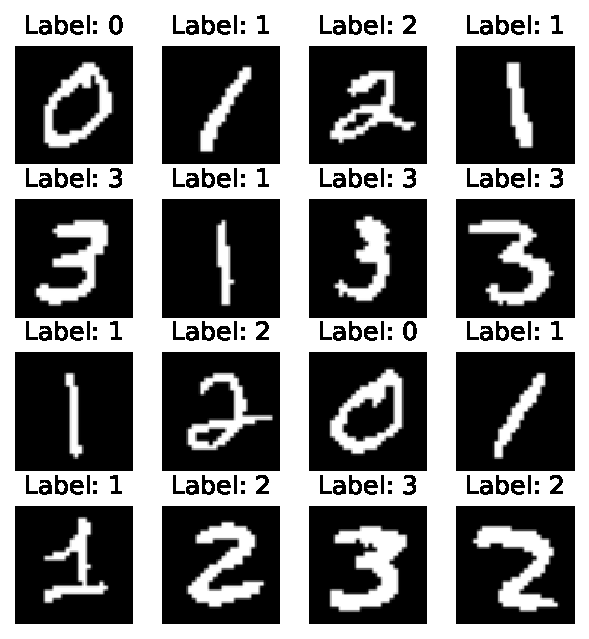
\includegraphics[scale=0.7]{latex/figures/bmnist.pdf}
\end{center}
\caption{Samples from the binarized MNIST dataset with labels 0-3.}
\label{fig:bmnist}
\end{figure}

\subsubsection{Simulated neural data}

We created a dataset of 10,000 simulated voltage traces from the Hodgkin-Huxley model using the following simulation protocol:

\begin{itemize}
    \item The active conductance parameters were sampled randomly to generate distinct voltage traces, with $\bar{g}_K \sim \mathrm{U} \qty(26, 46) \, \mathrm{mS/cm}^2$ and $\bar{g}_{Na} \sim \mathrm{U} \qty(110, 130) \,\mathrm{mS/cm}^2$.
    \item The rest of the model parameters were set to the values provided in \autoref{tab:hh_model_parameters}.
    \item In order to equilibrate the system, the system was first simulated for 200 ms without external stimuli. Then, we started recording and turned on a step current pulse with amplitude $I = 15 \, \mathrm{\mu A/cm}^2$ after 10 ms that lasted throughout the rest of the recorded simulation.
    \item We kept a recording of 50 ms. The time step of the simulation was 0.01 ms. This means that the time series we will train the VAEs on have a length of 5000 data points.
\end{itemize}

As a post-processing step, we applied min-max scaling to ensure voltage values on $[0, 1]$:

\begin{equation}
    V_\mathrm{scaled} = \frac{V - \min (V)}{\max(V) - \min(V)}
\end{equation}

8,000 of the simulation form the training set, and the remaining 2,000 the test set.

%----------------------------------------------------------------
\subsection{VAE models}
%----------------------------------------------------------------
\subsubsection{MLP- and DNN-VAE}

Our first model is a MLP-VAE, for which the encoder and decoder consists of an identical single hidden dense layer with the number of units set to 500. To investigate if there are some performance gains by using a slightly deeper dense network, we also build a DNN-VAE with 500 units in the first layer and 150 in the second of the encoder. The decoder of the DNN-VAE mirrors its encoder.

\subsubsection{Convolutional VAE}

We also built a convolutional VAE. The encoder network employs two convolutional layers, the first with 32 filters and the second 64, followed by a fully-connected layer. The decoder network mirrors this architecture by using a fully-connected layer followed by three convolution transpose layers in reverse order of the encoder.

\subsubsection*{Activation function and weight initialization}

As activation function, we use the Rectified Linear Unit (ReLU):

\begin{equation}
\mathrm{ReLU}(x) =\max( 0,\ x) 
\end{equation}

To maintain the variance of ReLU activations across layers, thereby preventing vanishing or exploding gradients, \cite{ReLu} showed that weights, $w$, should be initialized with values drawn from a normal distribution with a mean of 0 and a standard deviation of $\sqrt{\frac{2}{n_{in}}}$, where $n_{in}$ is the number of input units in the weight tensor. This is promptly known as He initialization.

%In the training neural networks, the initialization of weights is crucial for efficient learning and convergence. He initialization was employed to maintain the variance of activations across layers, thereby preventing vanishing or exploding gradients \citep{ReLu}. The weights $W$ are initialized with values drawn from a Gaussian distribution with a mean of 0 and a standard deviation of $\sqrt{\frac{2}{n_{in}}}$. The mathematical expression is given by

%\begin{equation*}
%W \sim \mathrm{N}\left(0, \frac{2}{n_{\text{in}}}\right)
%\end{equation*}

%where $n_{in}$ is the number of input units in the weight tensor. By utilizing He initialization in combination with the ReLu activation function, the network is able to train efficiently by maintaining the appropriate variance of activations and preventing issues related to gradient propagation. 

%\url{https://wandb.ai/sauravmaheshkar/initialization/reports/A-Gentle-Introduction-To-Weight-Initialization-for-Neural-Networks--Vmlldzo2ODExMTg}

\subsubsection{Latent distribution prior}

As prior on the latent distribution, $p(z)$, we choose the commonly used multivariate standard normal distribution:
\begin{equation*}
    p(z) = \mathrm{N} \qty(\mu=\bm{0}, \sigma^2=\bm{1})
\end{equation*}
This encourages encodings to distribute evenly around the center of the latent space.

%----------------------------------------------------------------
\subsection{Training the VAEs}
%----------------------------------------------------------------

\subsubsection{The NAdamW optimizer}

We use the NAdamW optimizer as the stochastic gradient descent method for updating the parameters of the VAE's encoder and decoder. NAdamW is an optimizer combining Adam \citep{kingma2017adam} with weight decay \citep{loshchilov2019decoupled}, then called AdamW, and momentum a la Nesterov introduced by \cite{dozat2016}. The weight decay regularize learning towards small weights, which leads to better generalization. 


Let $\alpha_t$ represent the learning rate, $\beta_1, \beta_2$ the exponential decay factors for the first and second moments, respectively, and $\varepsilon$, $\bar{\varepsilon}$ small constants applied to the denominator outside and inside, respectively, the square root to avoid dividing by zero when rescaling. The learning rate is
indexed by $t$ since the learning rate may also be provided by a
schedule function (see \autoref{sec:lr_schedule}). Let $\lambda$ be the weight decay and  $\theta_t$ the parameter vector at time $t$. The optimizers internal state $S_t := (m_t, v_t)$ represents the running average of the first and second moment of the gradient. We initialize the internal state as $S_0 = (m_0, v_0) = (0, 0)$. At step $t$, the optimizer takes incoming gradients $g_t$ and computes updates $u_t$ and the new state $S_{t+1}$. For $t > 0$, we have,


\begin{align*}
  m_t &\leftarrow \beta_1 \cdot m_{t-1} + (1-\beta_1) \cdot g_t \\
  v_t &\leftarrow \beta_2 \cdot v_{t-1} + (1-\beta_2) \cdot {g_t}^2 \\
  \hat{m}_t &\leftarrow \beta_1 m_t / {(1-\beta_1^{t+1})} + (1 - \beta_1) g_t / {(1-\beta_1^t)} \\
  \hat{v}_t &\leftarrow v_t / {(1-\beta_2^t)} \\
  u_t &\leftarrow -\alpha_t \cdot \left( \hat{m}_t / \left({\sqrt{\hat{v}_t 
  + \bar{\varepsilon}} + \varepsilon} \right) + \lambda \theta_{t} \right)\\
  S_t &\leftarrow (m_t, v_t).
\end{align*}


\subsubsection{Learning rate scheduler}\label{sec:lr_schedule}

The learning rate is one of the most important hyperparameters for training deep neural networks, as it determines the size of the steps taken during the optimization process. Instead of employing a fixed learning rate, it is common to dynamically adjust the learning rate during training according to a schedule. A learning rate scheduler can notably enhance convergence and overall model performance. In the training of the VAEs, we will use the \textit{cosine decay schedule} \citep{cosine_decay}. It starts with an initial learning rate and gradually decreases the learning rate following a cosine curve. The learning rate at iteration $t$ is given by

\begin{equation}\label{eq:cosine_decay}
    \frac{I \qty(1 - \alpha)}{2} \qty(1 + \cos \qty(\pi \frac{t}{T})^p) + \alpha,
\end{equation}

where $T$ is the number of decay steps, $p$ is an exponent that can be used to modify the decay curve, $I$ is the initial learning rate and $\alpha$ determines the final learning rate as a fraction of the initial learning rate. During training, we set 
\begin{align*}
    T &= \text{number of examples in a batch} \times \text{number of epochs}, \\
    p &= 1, \\
    I &= 10^{-3}, \\
    \intertext{and}
    \alpha &= 10^{-2}
\end{align*}
which means that the final learning rate will be $10^{-5}$. \autoref{fig:lr_schedule} illustrates the cosine decay scheduler.

\begin{figure}[!htb]
\begin{center}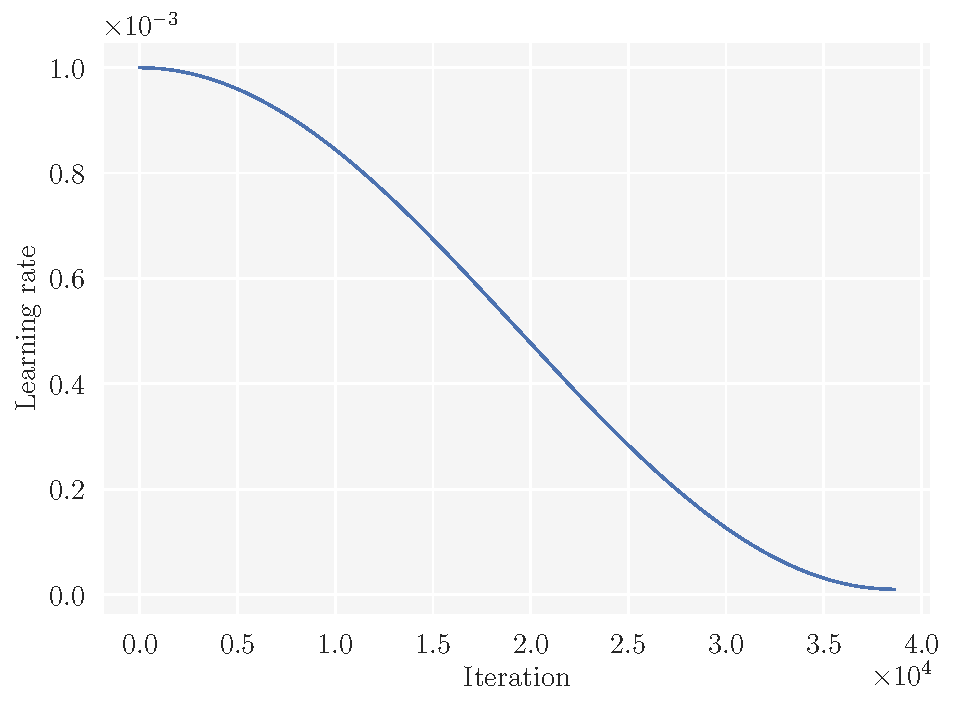
\includegraphics[scale=0.7]{latex/figures/lr_schedule.pdf}
\end{center}
\caption{Illustration of the cosine decay learning rate scheduler given by \autoref{eq:cosine_decay}. The variables of the cosine decay scheduler are set according to the description in the main text with 386 examples in one batch and 50 epochs.}
\label{fig:lr_schedule}
\end{figure}


\subsubsection{Loss functions}

For a standard normal prior, the KL-divergence (KLD) term of the ELBO becomes:

\begin{equation}
    D_{KL} \qty(q_\theta (z | x) || p(z)) = - \frac{1}{2}  \sum_j \qty(1 + \log \qty(\sigma_j^2) - \mu_j^2 - \sigma_j^2  )
\end{equation}

The reconstruction error of the binarized MNIST images is computed as the binary cross-entropy (BCE):

\begin{equation}
    BCE = - \frac{1}{n} \sum_{i=1}^n \qty(x_i \log \qty(\hat{x}_i) + \qty(1 - x_i) \log \qty(1-\hat{x}_i)  ),
\end{equation}

where $x_i$ is an original image and $\hat{x}_i$ its reconstruction. 

The reconstruction error of the simulated neural data is computed as the mean-squared error (MSE):

\begin{equation}
    MSE = \frac{1}{n} \sum_i^n \qty(x_i - \hat{x}_i)^2,
\end{equation}
where $x_i$ is the original signal and $\hat{x}_i$ the reconstruction.




